

\section{Summary of Proteome Datasets.}

[ NB: still very much in progress! ]

Here we briefly summarize the datasets that were considered for the work of the main
text. The goal of this section is to give an overview of each dataset
considered, including the main experimental details, and to provide a more
detailed look at how well each compares.

Table \ref{table:datasets} provides an overview of the proteomic datasets that
we found in the literature. These are predominately mass spectrometry-based,
with the exception of the work from Li \textit{et al.} (2014) which used ribosomal
profiling, and the fluorescence-based counting done in Taniguchi \textit{et al.}
(2010). The general strategy taken in these works is to quantify fractional
abundance of each protein and then to convert these to absolute abundance by
multiplying these fractions by the bulk measured total cellular protein
abundance. Note that the work of Peebo \textit{et al.} (2014) did not perform any
measurement of cell count or volume, and thus were only able to report cellular
protein concentration.

Exceptions to this are found in Schmidt \textit{et al.} and Taniguchi \textit{et al.}.
A key distinction in the work of Schmidt \textit{et al.} is that in addition to
determining relative abundance by mass spectrometry, they also selected 41
enzyme that cover over four orders of magnitude in cellular abundance to use in
absolute protein quantification. Specifically, synthetic peptides were generated
for each of these 41 enzymes and used to provide a calibration between measured
mass spectrometry intensities and absolute protein abundances (using stable
isotope dilution (SID) and selected reaction monitoring (SRM), though the
details of this are beyond the scope of this section). In the work of Taniguchi
\textit{et al.},  the authored tagged each protein with a  yellow fluorescent
protein (YFP) and used fluorescence as readout of cellular expression.


% \begin{center}
\begin{tabularx}{.8\textwidth}{ || c | c | c | c | c | c | c || }
\hline
Author & Method & Strain & $N$ datasets & Reported Quantity & fractional coverage (by count) & fractional coverage (by mass) \\
\hline\hline
Taniguchi \textit{et al.} (2010) & YFP-fusion, cell fluorescence  & & & fg/copies per cell & & \\
\hline
Valgepea \textit{et al.} (2012) & Mass spectrometry  & & & fg/copies per cell & & \\
\hline
Peebo \textit{et al.} (2014) & Mass spectrometry  & & & fg/copies per fl & & \\
\hline
Li \textit{et al.} (2014) & Ribosomal profiling  & & & protein synthesis rate & & \\
\hline
Soufi \textit{et al.} (2015) & Mass spectrometry  & & & fg/copies per cell & &\\
\hline
Schmidt \textit{et al.} (2016) & Mass spectrometry  & & & fg/copies per cell & & \\
\hline
Caglar \textit{et al.} (2017) & Mass spectrometry  & & & relative abundance & &\\
\hline
\end{tabularx}
% \label{table:datasets}
% \end{center}

Figure \ref{} shows the distribution in reported protein abundance for   a  subset
of  the data.

An important consideration is whether the reported abundance per cell are correlated. while
we expect some variability in expression of each protein due to growth rate, the reported
values are nonetheless expected to be correlated. Figure \ref{fig:dataset_correlations} compares each dataset to the copy numbers from Schmidt \textit{et al.}, grown in M9 minimal media supplemented with glucose.
%
% \begin{figure}[H]
% 		\centering
%     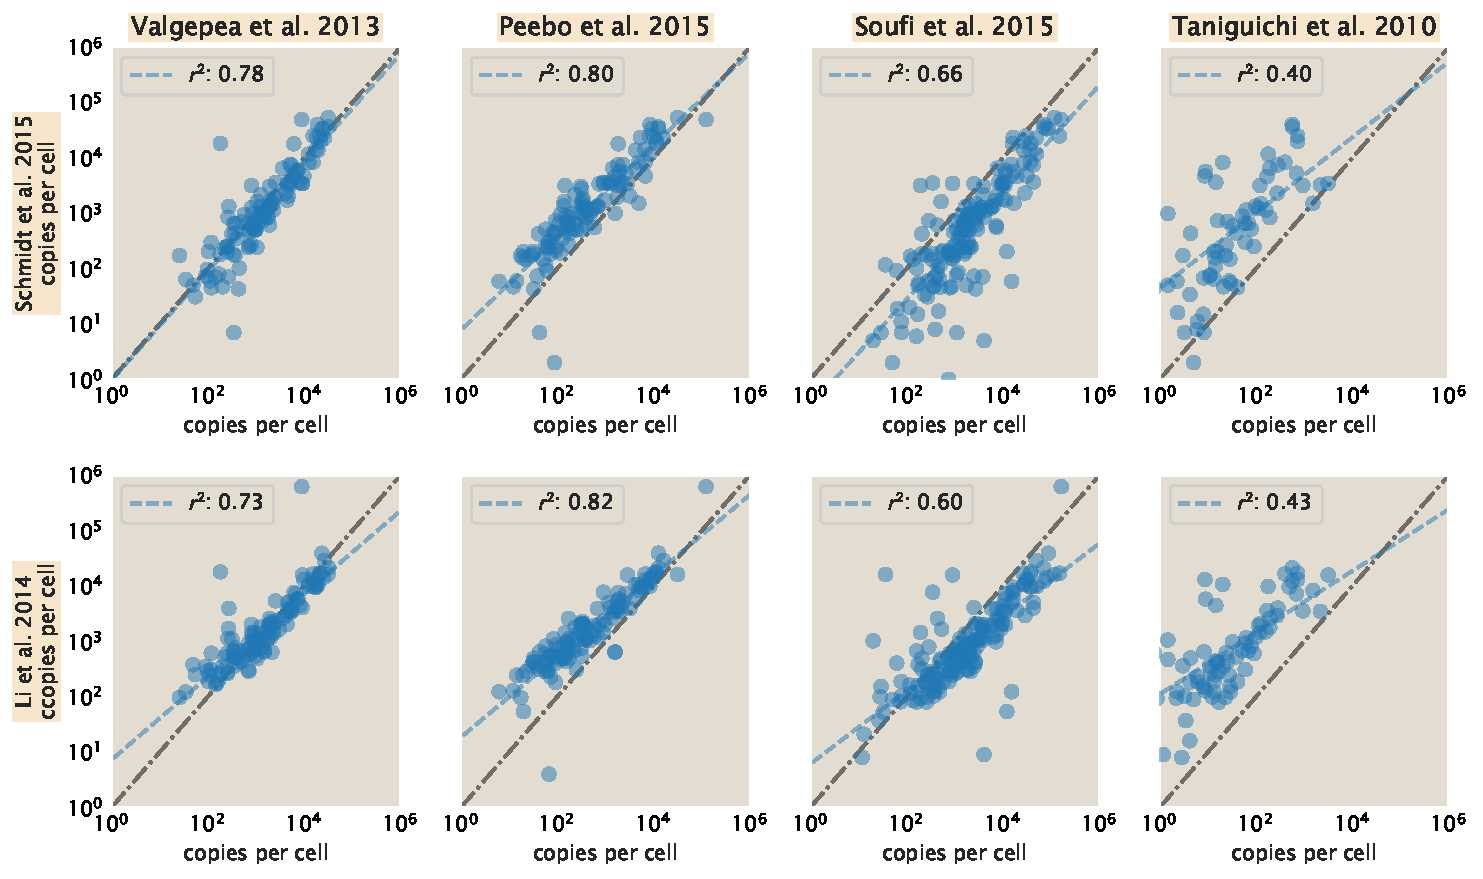
\includegraphics[width=1\textwidth]{../../figures/dataset_correlations.pdf}
%   \caption{}
%   \label{fig:dataset_correlations}
% \end{figure}
%
% \begin{figure}[H]
% 		\centering
%     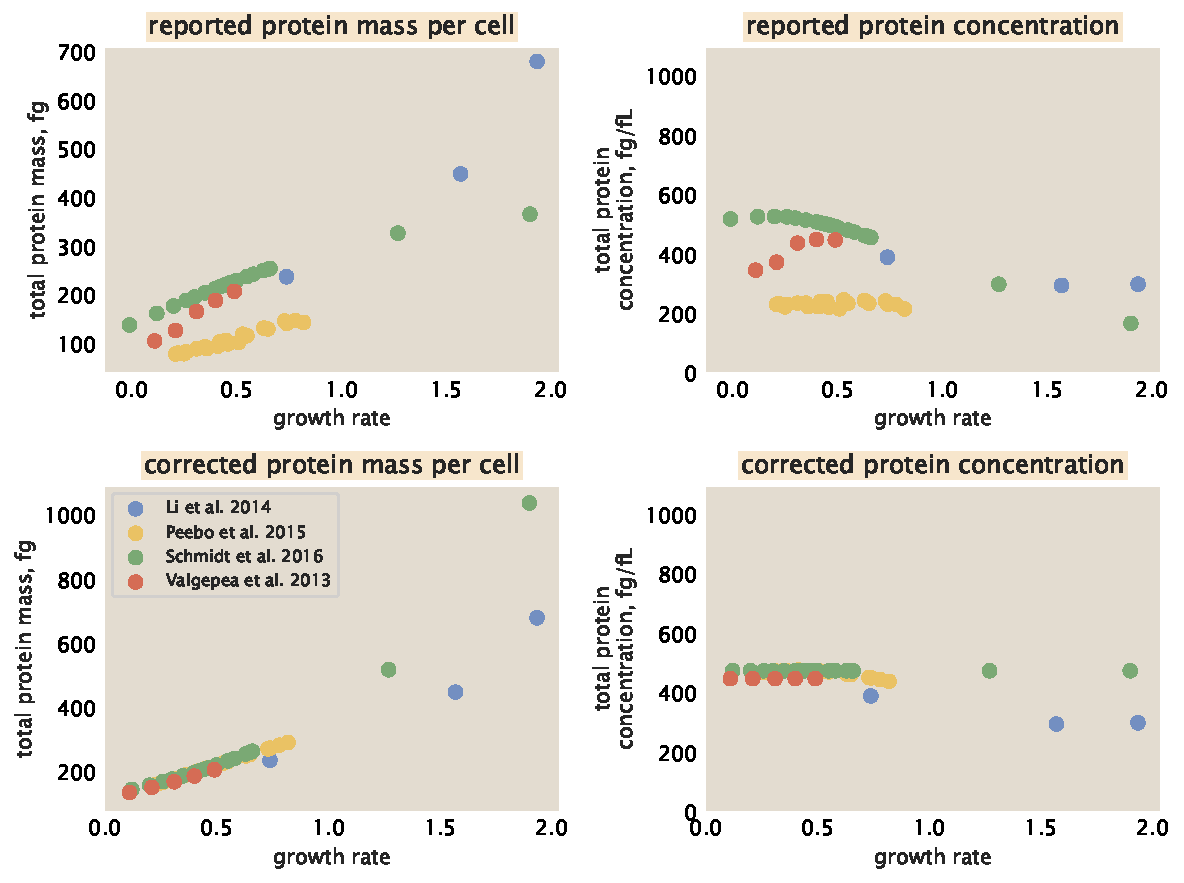
\includegraphics[width=1\textwidth]{../../figures/dataset_corrections.pdf}
%   \caption{}
%   \label{fig:dataset_correlations}
% \end{figure}
%
